\chapter{Perancangan Perangkat Lunak}
\label{chap:perancangan}

Pada bab ini akan dijabarkan perancangan perangkat lunak untuk penelitian ini. Perancangan perangkat lunak tersebut meliputi perancangan antarmuka dan perancangan kelas untuk penelitian ini.

\section{Perancangan Antarmuka}
\label{sec:antarmuka}

Perancangan antarmuka yang dibuat disesuaikan dengan diagram kelas dan diagram aktivitas yang dibuat sesuai analisis perangkat lunak dilakukan. Perangkat lunak randomisasi akan memiliki 3 halaman antarmuka yang diimplementasikan dengan desain antarmuka tabs. Rancangan antarmuka halaman utama dapat dilihat pada Gambar ~\ref{fig:hal-awal}, halaman ini akan berisi pesan selamat datang berupa deskripsi singkat perangkat lunak beserta cara kerjanya dan petunjuk singkat cara penggunaan perangkat lunak. Pada bagian atas antarmuka terdapat sebuah kolom untuk memasukkan file csv yang ingin dirandomisasi. Pertama-tama pengguna wajib untuk mengisi kolom tersebut apapun teknik randomisasi yang akan digunakan nanti.

Setelah pengguna memasukkan file yang diinginkan, perangkat lunak akan menampilkan berbagai informasi mengenai dataset yang ada di file tersebut seperti ukuran filenya, nama filenya, dan jumlah kolom. Deskripsi ini bertujuan untuk memberitahukan pengguna bahwa file yang dimasukkan telah benar dan bagaimana sifat dari dataset yang dimasukkan. 

\begin{figure}
	\centering
	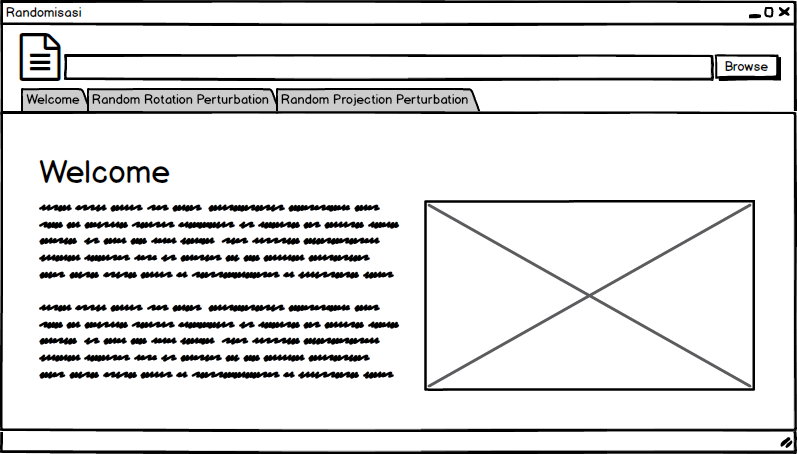
\includegraphics[scale=0.56]{hal-awal}
	\caption{Halaman utama yang berisi petunjuk cara penggunaan perangkat lunak}
	\label{fig:hal-awal}
\end{figure}

\subsection{Halaman \textit{Random Rotation Perturbation}}
\label{subsec:tabrrp}

Halaman ini memiliki fungsi untuk melakukan teknik \textit{Random Rotation Perturbation}. Setelah user memasukkan file yang diinginkan pada kolom yang berada pada bagian atas antarmuka, pengguna baru bisa mengakses halaman ini. Pada halaman ini terdapat berbagai informasi dataset yang dimasukkan dan hasil dari randomisasi jika berhasil dilakukan, serta pengaturan apa saja fitur yang akan dirandomisasi pada dataset yang pengguna masukkan. Rancangan dari halaman ini dapat dilihat pada Gambar ~\ref{fig:tab-rrp}.

\begin{figure}
	\centering
	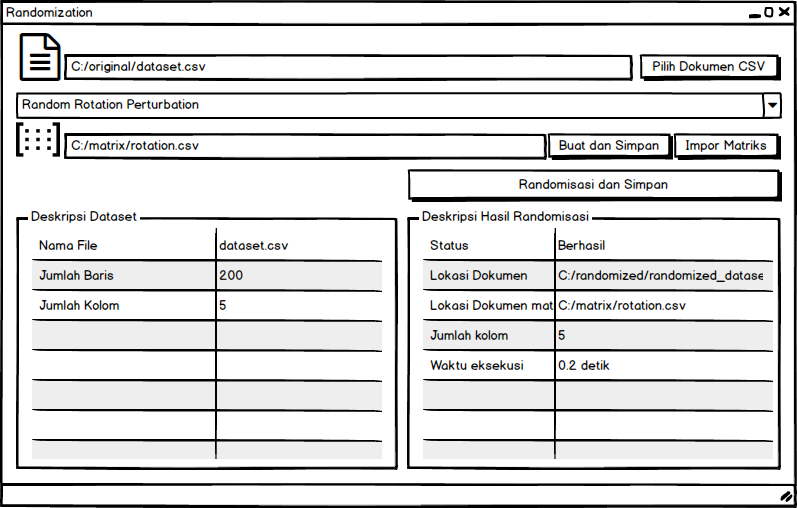
\includegraphics[scale=0.56]{tab-rrp}
	\caption{Halaman untuk melakukan teknik \textit{Random Rotation Perturbation}}
	\label{fig:tab-rrp}
\end{figure}

Sebelum melakukan randomisasi, pengguna perlu memeriksa fitur mana saja yang ingin dirandomisasi karena bisa saja pada dataset tersebut ada kolom yang berupa label. Perangkat lunak akan menyimpan hasil randomisasi pada file dataset pengguna yang telah diubah nilainya dan perangkat lunak akan menyimpan file tersebut di suatu lokasi yang pengguna harus tentukan. Pengguna bisa menentukan lokasi file hasil randomisasi pada kolom yang terdapat di sebelah kanan ikon simpan dan sebelah kiri tombol "Randomisasi dan Simpan".

Setelah pengguna melakukan berbagai pengaturan, pengguna dapat melakukan randomisasi dengan menekan tombol "Randomisasi dan Simpan". Apabila randomisasi berhasil dilakukan, perangkat lunak akan menampilkan \textit{popup} yang memberitahukan bahwa randomisasi dengan teknik \textit{Random Rotation Perturbation} pada dataset yang dimasukkan berhasil dilakukan. \textit{Popup} tersebut dapat dilihat pada Gambar ~\ref{fig:popup-sukses}. Selain itu, perangkat lunak juga akan menampilkan berbagai informasi beserta deskripsi tentang hasil randomisasi yang berhasil dilakukan.

\begin{figure}
	\centering
	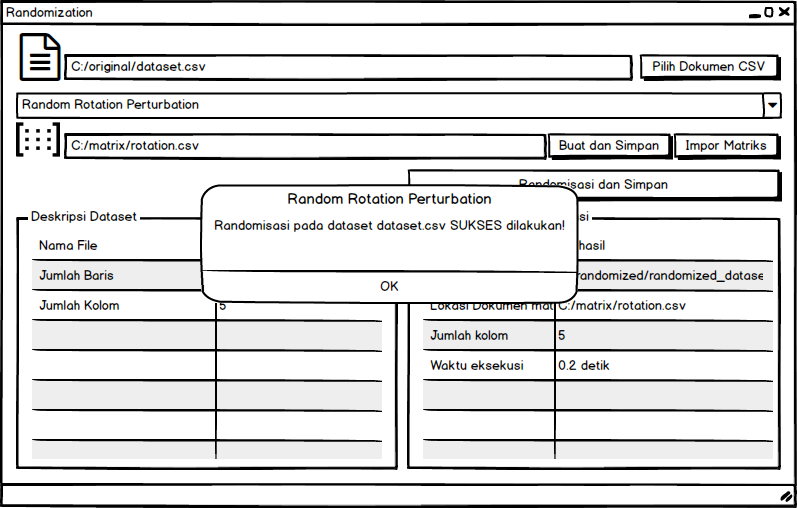
\includegraphics[scale=0.56]{popup-sukses}
	\caption{\textit{Popup} yang ditampilkan apabila randomisasi sukses dilakukan}
	\label{fig:popup-sukses}
\end{figure}

Perangkat lunak akan menampilkan deskripsi hasil dari randomisasi yang dilakukan. Informasi yang ditampilkan oleh perangkat lunak antara lain nama file, ukuran file, jumlah fitur, dan kolom yang diabaikan. Informasi ini ditampilkan oleh perangkat lunak bertujuan untuk memberitahukan pengguna properti-properti dataset yang telah dirandomisasi dan pengguna dapat memeriksa hasil yang dihasilkan oleh perangkat lunak apakah sesuai dengan keinginan pengguna.

Apabila ada masalah-masalah tertentu dan randomisasi gagal dilakukan, maka perangkat lunak akan memberitahukan bahwa randomisasi telah gagal dilakukan dengan menampilkan \textit{popup} yang berisi peringatan bahwa randomisasi gagal dilakukan. Hasil randomisasi tidak akan terbuat dan perangkat lunak tidak akan menampilkan informasi apapun tentang hasil randomisasi. \textit{Popup} tersebut dapat dilihat pada Gambar ~\ref{fig:popup-gagal}.

\begin{figure}
	\centering
	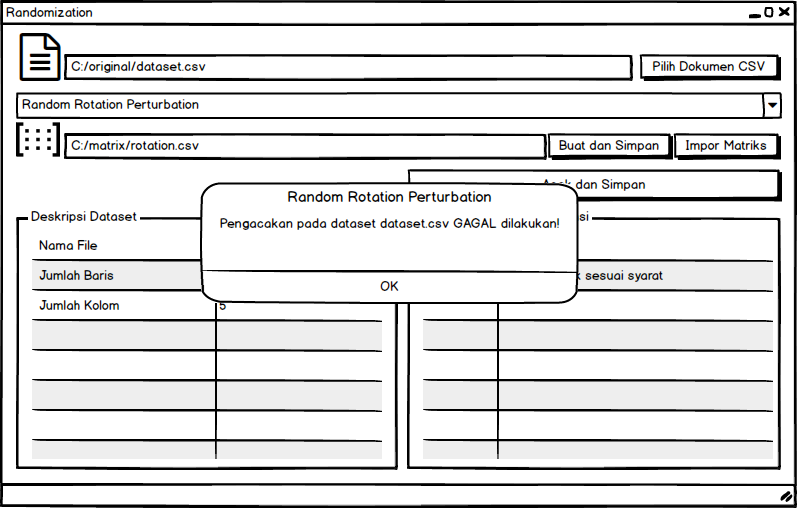
\includegraphics[scale=0.56]{popup-gagal}
	\caption{\textit{Popup} yang ditampilkan apabila randomisasi gagal dilakukan}
	\label{fig:popup-gagal}
\end{figure}

\subsection{Halaman \textit{Random Projection Perturbation}}
\label{subsec:tabrpp}

Halaman ini memiliki fungsi untuk melakukan teknik \textit{Random Projection Perturbation}. Rancangan dari halaman ini dapat dilihat pada Gambar ~\ref{fig:tab-rpp}. Sebelum pengguna melakukan randomisasi, pengguna harus mengatur beberapa pengaturan yang ada. Sama seperti halnya pada halaman \textit{Random Rotation Perturbation}, pengguna perlu menentukan lokasi penyimpanan hasil randomisasi yang akan dilakukan dan kolom apa saja pada dataset yang menjadi fitur. Pada bagian pemilihan fitur pada dataset, perangkat lunak mempunyai fitur kolom pencarian untuk mencari fitur pada dataset secara mudah dengan mengetikkan nama fitur yang diinginkan.

Selain itu, pada halaman ini yang khusus untuk teknik \textit{Random Projection Perturbation} pengguna harus menentukan dimensi yang diinginkan dan nilai epsilon. Setelah pengaturan-pengaturan tersebut diatur, pengguna dapat melakukan randomisasi menggunakan teknik \textit{Random Projection Perturbation} dengan menekan tombol "Randomisasi dan Simpan", perangkat lunak akan melakukan randomisasi dan menyimpan hasil randomisasi di lokasi yang telah pengguna tentukan. 

Pada teknik \textit{Random Projection Perturbation}, ada persyaratan yang harus dipenuhi mengenai dimensi akhir yang diinginkan dan nilai epsilon. Kedua nilai tersebut perlu sesuai dengan dataset yang ada sehingga pengguna tidak bisa sembarangan menentukan dimensi dan nilai epsilon. Perangkat lunak akan membuat aturan mengenai minimal dimensi yang bisa digunakan sehingga pengguna tidak bisa memasukan dimensi yang lebih kecil dari minimal yang telah ditentukan. Minimal dimensi ini bergantung pada banyaknya baris pada dataset dan nilai epsilon seperti yang telah dijelaskan pada bagian analisis bab 3.

Apabila randomisasi berhasil dilakukan, maka perangkat lunak akan menampilkan beberapa deskripsi tentang hasil randomisasi yang berhasil dilakukan seperti nama file hasil randomisasi, ukuran file, nilai epsilon yang dipakai, jumlah dimensi pada hasil randomisasi, dan kolom-kolom apa saja yang diabaikan. Perangkat lunak juga akan menyimpan hasil randomisasi yang telah dilakukan dalam bentuk file csv di lokasi yang telah ditentukan sebelumnya oleh pengguna.

\begin{figure}
	\centering
	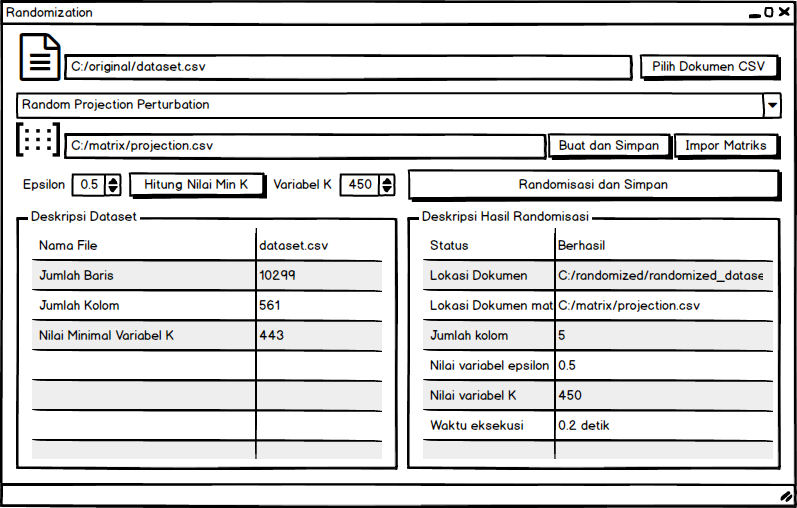
\includegraphics[scale=0.56]{tab-rpp}
	\caption{Halaman untuk melakukan teknik \textit{Random Projection Perturbation}}
	\label{fig:tab-rpp}
\end{figure}

Oleh karena adanya persyaratan yang harus dipenuhi oleh pengguna untuk melakukan randomisasi dengan teknik \textit{Random Projection Perturbation}, maka randomisasi bisa saja gagal dilakukan karena persyaratan yang ada tidak dipenuhi oleh pengguna. Persyaratan yang disebutkan adalah persyaratan jumlah dimensi dan nilai epsilon yang telah dijelaskan di atas. Perangkat lunak akan menampilkan \textit{popup} yang memberitahukan bahwa persyaratan tidak dipenuhi dan pengguna harus mengatur kembali pengaturan atau mengganti dataset. Rancangan ini dapat dilihat pada Gambar ~\ref{fig:popup-syarat}.

\begin{figure}
	\centering
	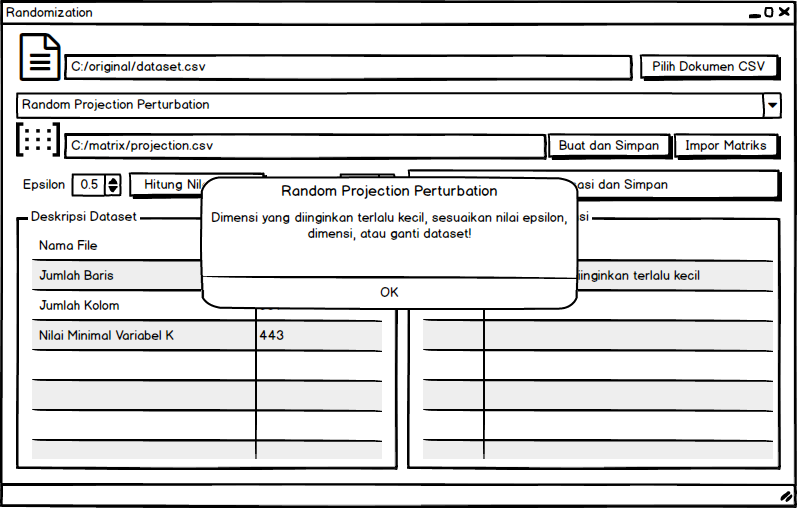
\includegraphics[scale=0.56]{popup-syarat}
	\caption{\textit{Popup} yang akan ditampilkan apabila syarat pada dataset tidak terpenuhi}
	\label{fig:popup-syarat}
\end{figure}

\section{Perancangan Kelas}
\label{sec:kelas}

<<TODO>>
